\documentclass[10pt]{article}
\usepackage[numbers]{natbib}
\usepackage[margin=1in]{geometry}
\usepackage{amsmath,amsthm,amssymb}
\usepackage{graphicx}
\usepackage{float}

\title{Modeling Click Prediction with Assortment}
\author{Juan Muneton Gallego}
\date{}
\begin{document}
\maketitle

\section*{Introduction}
Artificial Intelligence has revolutionized e-commerce by enabling businesses to better understand customer behavior, optimize recommendations, and personalize user experiences. Through large-scale analysis of user interactions, AI systems can uncover nuanced relationships between user intent and product relevance. Among the most impactful applications is click prediction \cite{Bai_Geng_Deng_Xia_Jiang_Yan_Liang_2025}, which anticipates which product a user is most likely to engage with given their query and the available assortment.

In this project, we focus on click prediction with assortment in the context of online wine purchasing. The goal is to predict which wine a user will most likely click on from a set of candidate bottles shown in response to their query. To this end, we attempt to fine-tune RoBERTa-based cross-encoder models \cite{liu2019robertarobustlyoptimizedbert} that jointly encode the user query and each wine's description to capture deep semantic relationships between intent and product attributes with the goal of improving ranking relevance and personalization in wine recommendations.

\section*{Methodology}
\subsection*{Datasets}
The datasets used in this project comprise user click-stream data and detailed product information related to wine purchases. The click dataset includes 12,932 queries in the training set and 3,233 in the test set, where each query corresponds to a user's search accompanied by an assortment of candidate wine products and a single binary label identifying the clicked item. This means that exactly one product per query is marked as relevant (clicked), while all others are treated as non-relevant, forming a one-hot encoded target vector as the labels. The number of suggested wines per query varies between 1 and 32, capturing diverse search contexts and assortment sizes. The accompanying catalog dataset provides textual descriptions and metadata for 2,600 unique wine products.

\subsection*{Data Preprocessing}
The preprocessing pipeline merges the training queries and test queries with the product catalog. Each query record contains a list of candidate product IDs in the \texttt{results} column and corresponding click labels in the \texttt{new\_labels} column. The catalog dataset provides detailed product information indexed by \texttt{WineID}.

\begin{sloppypar}
In the integration process of the datasets, we created a lookup dictionary mapping each \texttt{WineID} to its corresponding \texttt{product\_\allowbreak{}embed\_\allowbreak{}description} text from the catalog. For each query, candidate product IDs are resolved through this dictionary to retrieve their textual descriptions, which serve as input to the ranking model.
\end{sloppypar}

Query-product pairs are tokenized using the RoBERTa-base tokenizer. For each query $q_i$ with $N_i$ wine candidates, the pipeline constructs $N_i$ text pairs by concatenating the query with each product description. These pairs are tokenized with a maximum sequence length of 256 tokens, using truncation without padding to preserve the true sequence lengths. Eventually, the sequences are stored in their unpadded form in the Parquet files. This design choice significantly reduces storage requirements and I/O overhead, as padding to a global maximum would waste substantial disk space given the variability in both candidate set sizes (1-32 products per query) and sequence lengths. The sequence padding is deferred to batch construction time via a custom collation function.

The training data undergoes a random 90-10 split with seed 42 for reproducibility, generating separate training and validation sets. The test set remains intact without splitting. All processed data is serialized to Apache Parquet format with ZSTD compression.

Each preprocessed record contains: (1) \texttt{input\_ids} -- a list of $N$ tokenized sequences, (2) \texttt{attention\_mask} -- corresponding attention masks, (3) \texttt{label\_index} -- the index of the clicked product (obtained via argmax over the one-hot encoded labels), and (4) \texttt{n\_candidates} -- the number of products per query.

During training, the custom collation function implements variable-length batch processing to handle the inherent variability in candidate set sizes and sequence lengths across queries. For each batch of $B$ queries, the collator pads both the candidate dimension (to $\max_N$) and token dimension (to $\max_L$) dynamically, ensuring memory efficiency by avoiding unnecessary padding beyond the batch maximum. A binary \texttt{candidate\_mask} of shape $[B, \max_N]$ distinguishes real candidates from padding, enabling proper masking during model computation. 
\subsection*{Model Architectures}
We fine-tune three variants of a RoBERTa-based cross-encoder architecture, each differing in how token-level representations are aggregated into a fixed-dimensional query-product relevance score. All models share a common structure: a pretrained RoBERTa-base backbone encoder (with hidden dimension $d=768$). The final pooled representation is passed through a linear classification head that outputs a single relevance score per query-product pair. The three pooling strategies explored are: (1) standard CLS token, (2) mean pooling across all tokens, and (3) attention-based pooling with learned weights.

\subsubsection*{Cross-Encoder with CLS }
The baseline model uses the standard CLS token pooling strategy, where only the final hidden state corresponding to the special \texttt{[CLS]} token is extracted and passed through the classification head. This approach relies on the transformer's ability to encode the entire sequence's semantic information into the first token position through self-attention. 

\subsubsection*{Cross-Encoder with Mean Pooling}
While computationally efficient and widely adopted in sentence-pair classification tasks, CLS pooling may underutilize information from other token positions, particularly in cases where product descriptions contain rich, fine-grained details relevant to the query. Therefore another alternative that we explored is the mean pooling variant. This model computes the element-wise average of all token representations, weighted by the attention mask to exclude padding tokens \cite{xing2025comparativeanalysispoolingmechanisms}. Formally, for a sequence of length $L$ with hidden states $H \in \mathbb{R}^{L \times d}$ and attention mask $m \in \{0,1\}^L$, the pooled representation is:
\[
h_{\text{pool}} = \frac{\sum_{i=1}^{L} m_i h_i}{\sum_{i=1}^{L} m_i}
\]
This method captures global semantic information by aggregating contributions from all tokens uniformly.

\subsubsection*{Cross-Encoder with Attention Pooling}
In the previous subsection, we introduced mean pooling as a way to aggregate token representations. However, mean pooling assumes that all tokens contribute equally to the final representation, which may not be optimal for tasks where certain tokens carry more significance than others. To address this limitation, we implement an attention pooling mechanism that learns to weight token contributions based on their relevance to the classification task.
This method introduces a learned weighting mechanism to selectively aggregate token representations based on their relevance to the classification task \cite{santos2016attentivepoolingnetworks}. The pooling layer consists of two linear transformations: $W_1 \in \mathbb{R}^{d \times d}$ and $W_2 \in \mathbb{R}^{1 \times d}$. For each token's hidden state $h_i$, attention scores are computed as:
\[
s_i = W_2 \left( \tanh(W_1 h_i) \right)
\]
These scores are masked to exclude padding tokens, then normalized via softmax to produce attention weights $\alpha_i$. The final pooled representation is:
\[
h_{\text{pool}} = \sum_{i=1}^{L} \alpha_i h_i
\]
This adaptive pooling strategy allows the model to dynamically emphasize tokens that are most discriminative for predicting click relevance.
\subsection*{Training/Fine-Tuning Procedures}
All models are fine-tuned for 7 epochs with a batch size of 16 and a learning rate of $2 \times 10^{-5}$. We employ the AdamW optimizer \cite{loshchilov2019decoupledweightdecayregularization} with a weight decay of 0.01 for regularization. To stabilize early training, a linear warmup schedule is applied over the first 500 optimization steps, after which the learning rate follows a cosine annealing decay \cite{loshchilov2017sgdrstochasticgradientdescent} to zero over the remaining training steps. Gradients are clipped to a maximum norm of 1.0 to prevent training instability.

\subsubsection*{Loss Function}
The models were fine-tuned using cross-entropy loss over the candidate set for each query. Given a batch of $B$ queries, each with $N_b$ candidates, the model produces a score vector $\mathbf{s}_b \in \mathbb{R}^{N_b}$ for query $b$. These scores are masked to exclude padded candidates using the candidate mask $m_b$, setting scores for invalid positions to $-\infty$ before applying softmax. The cross-entropy loss is computed between the resulting probability distribution and the ground-truth label index $y_b$:
\[
\mathcal{L} = -\frac{1}{B} \sum_{b=1}^{B} \log \frac{\exp(s_{b, y_b})}{\sum_{i=1}^{N_b} m_{b,i} \exp(s_{b,i})}
\]
This formulation treats click prediction as a single-label classification problem, where exactly one product per query is relevant.

Cross-entropy loss measures the divergence between the predicted probability distribution over candidates and the ground-truth distribution (which assigns probability 1 to the clicked item and 0 to all others). Note that lower cross-entropy values indicate that the model assigns higher probability mass to the correct product.
\subsubsection*{Hardware}
The experiments were performed on an NVIDIA RTX PRO 6000 GPU (95.6~GB VRAM, 119~TFLOPS, CUDA~13.0) paired with an AMD EPYC~9B14~96-core CPU and~96.7~GB of RAM. The environment was built on the \texttt{vastai/base-image\_cuda-13.0.1-auto/jupyter} container, running PyTorch with mixed-precision training enabled.

\subsubsection*{Optimization Strategies}
All models were fine-tuned with FP16 mixed precision using automatic mixed precision (AMP). We applied differential learning rates: the RoBERTa backbone is trained at the base learning rate of $2 \times 10^{-5}$, while the classification head receives a 5x higher learning rate of $1 \times 10^{-4}$ to facilitate faster adaptation of the task-specific layer.

\subsubsection*{Summary of Hyperparameters}
Table \ref{tab:hyperparameters} summarizes the key hyperparameters used across all experiments.

\begin{table}[H]
\centering
\caption{Training hyperparameters}
\label{tab:hyperparameters}
\begin{tabular}{lr}
\hline
\textbf{Hyperparameter} & \textbf{Value} \\
\hline
Number of Epochs & 7 \\
Batch Size & 16 \\
Base Learning Rate (Backbone) & $2 \times 10^{-5}$ \\
Head Learning Rate & $1 \times 10^{-4}$ \\
Weight Decay & 0.01 \\
Warmup Steps & 500 \\
LR Schedule & Cosine Annealing \\
Gradient Clipping & 1.0 \\
Max Sequence Length & 256 \\
Optimizer & AdamW \\
\hline
\end{tabular}
\end{table}
\subsection*{Evaluation Metrics}
Model performance is assessed using two complementary metrics: cross-entropy loss and classification accuracy. 


\section*{Results}
Across all evaluated architectures, the Cross-Encoder models achieved comparable performance, with test accuracies ranging between 0.533 and 0.541. The Mean Pooling variant obtained the highest test accuracy (0.541), though its loss was slightly higher than the others, suggesting less confident but more calibrated predictions. The Attention Pooling model yielded the lowest test loss (1.772). See table \ref{tab:model_performance} for details.
\begin{table}[H]
\centering
\caption{Model performance comparison on the test set.}
\label{tab:model_performance}
\begin{tabular}{lcc}
\hline
\textbf{Model Name} & \textbf{Test Loss} & \textbf{Test Accuracy} \\
\hline
Cross-Encoder (CLS Pooling) & 1.798 & 0.539 \\
Cross-Encoder (Mean Pooling) & 1.948 & 0.541 \\
Cross-Encoder (Attention Pooling) & 1.772 & 0.533 \\
\hline
\end{tabular}
\end{table}
\subsection*{Cross-Encoder with CLS Pooling}
Figure \ref{fig:combined_cls} shows the training and validation performance over epochs for the CLS pooling model, while Figure \ref{fig:step_cls} presents the step-level training dynamics.

\begin{figure}[H]
\centering
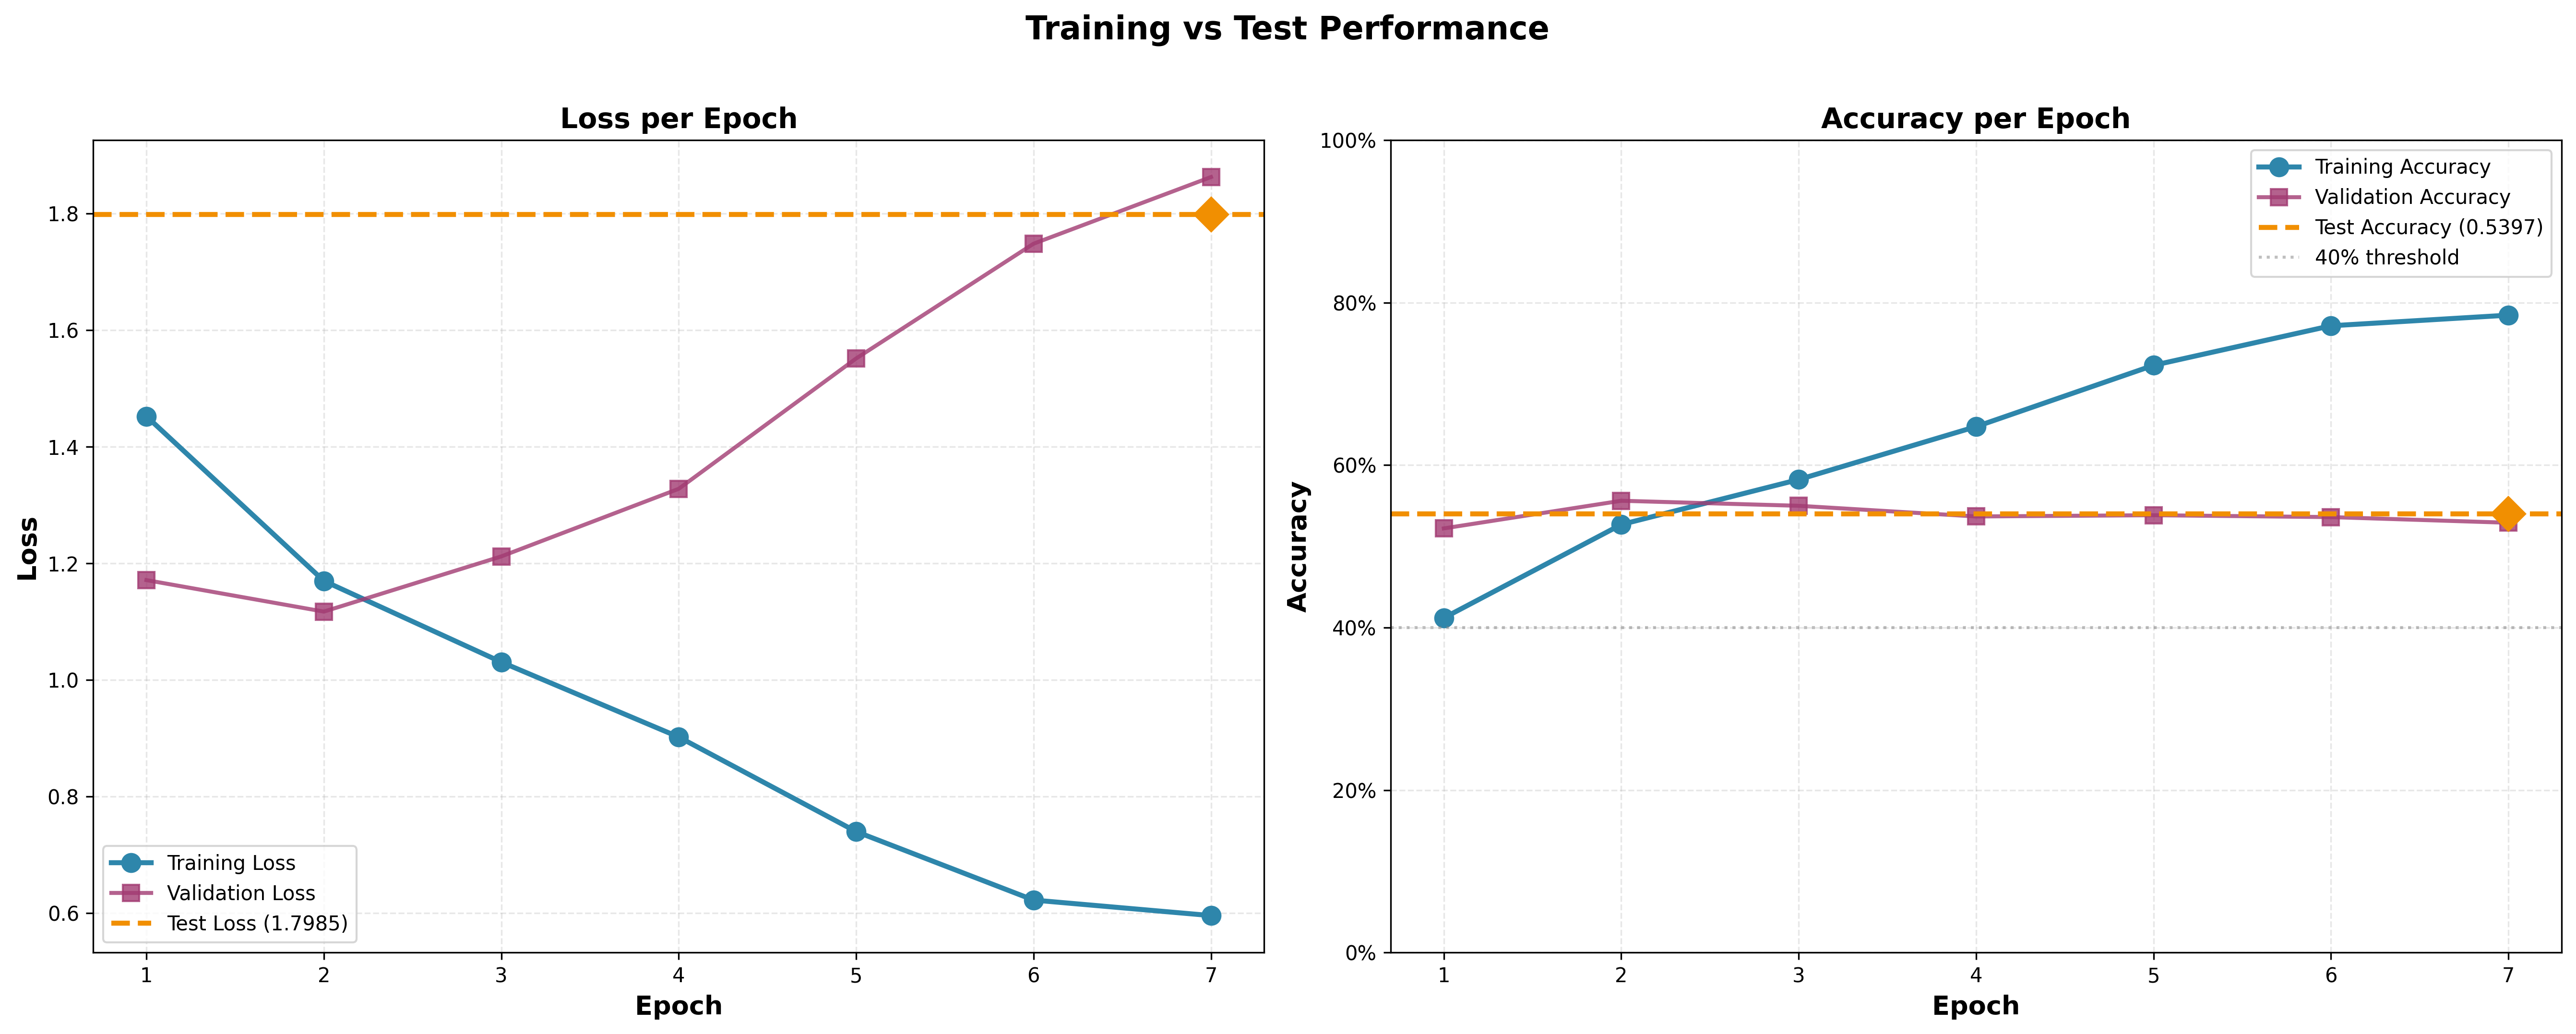
\includegraphics[width=0.85\textwidth]{combined_plot_cls.png}
\caption{Training and validation metrics across epochs for Cross-Encoder with CLS Pooling.}
\label{fig:combined_cls}
\end{figure}

\begin{figure}[H]
\centering
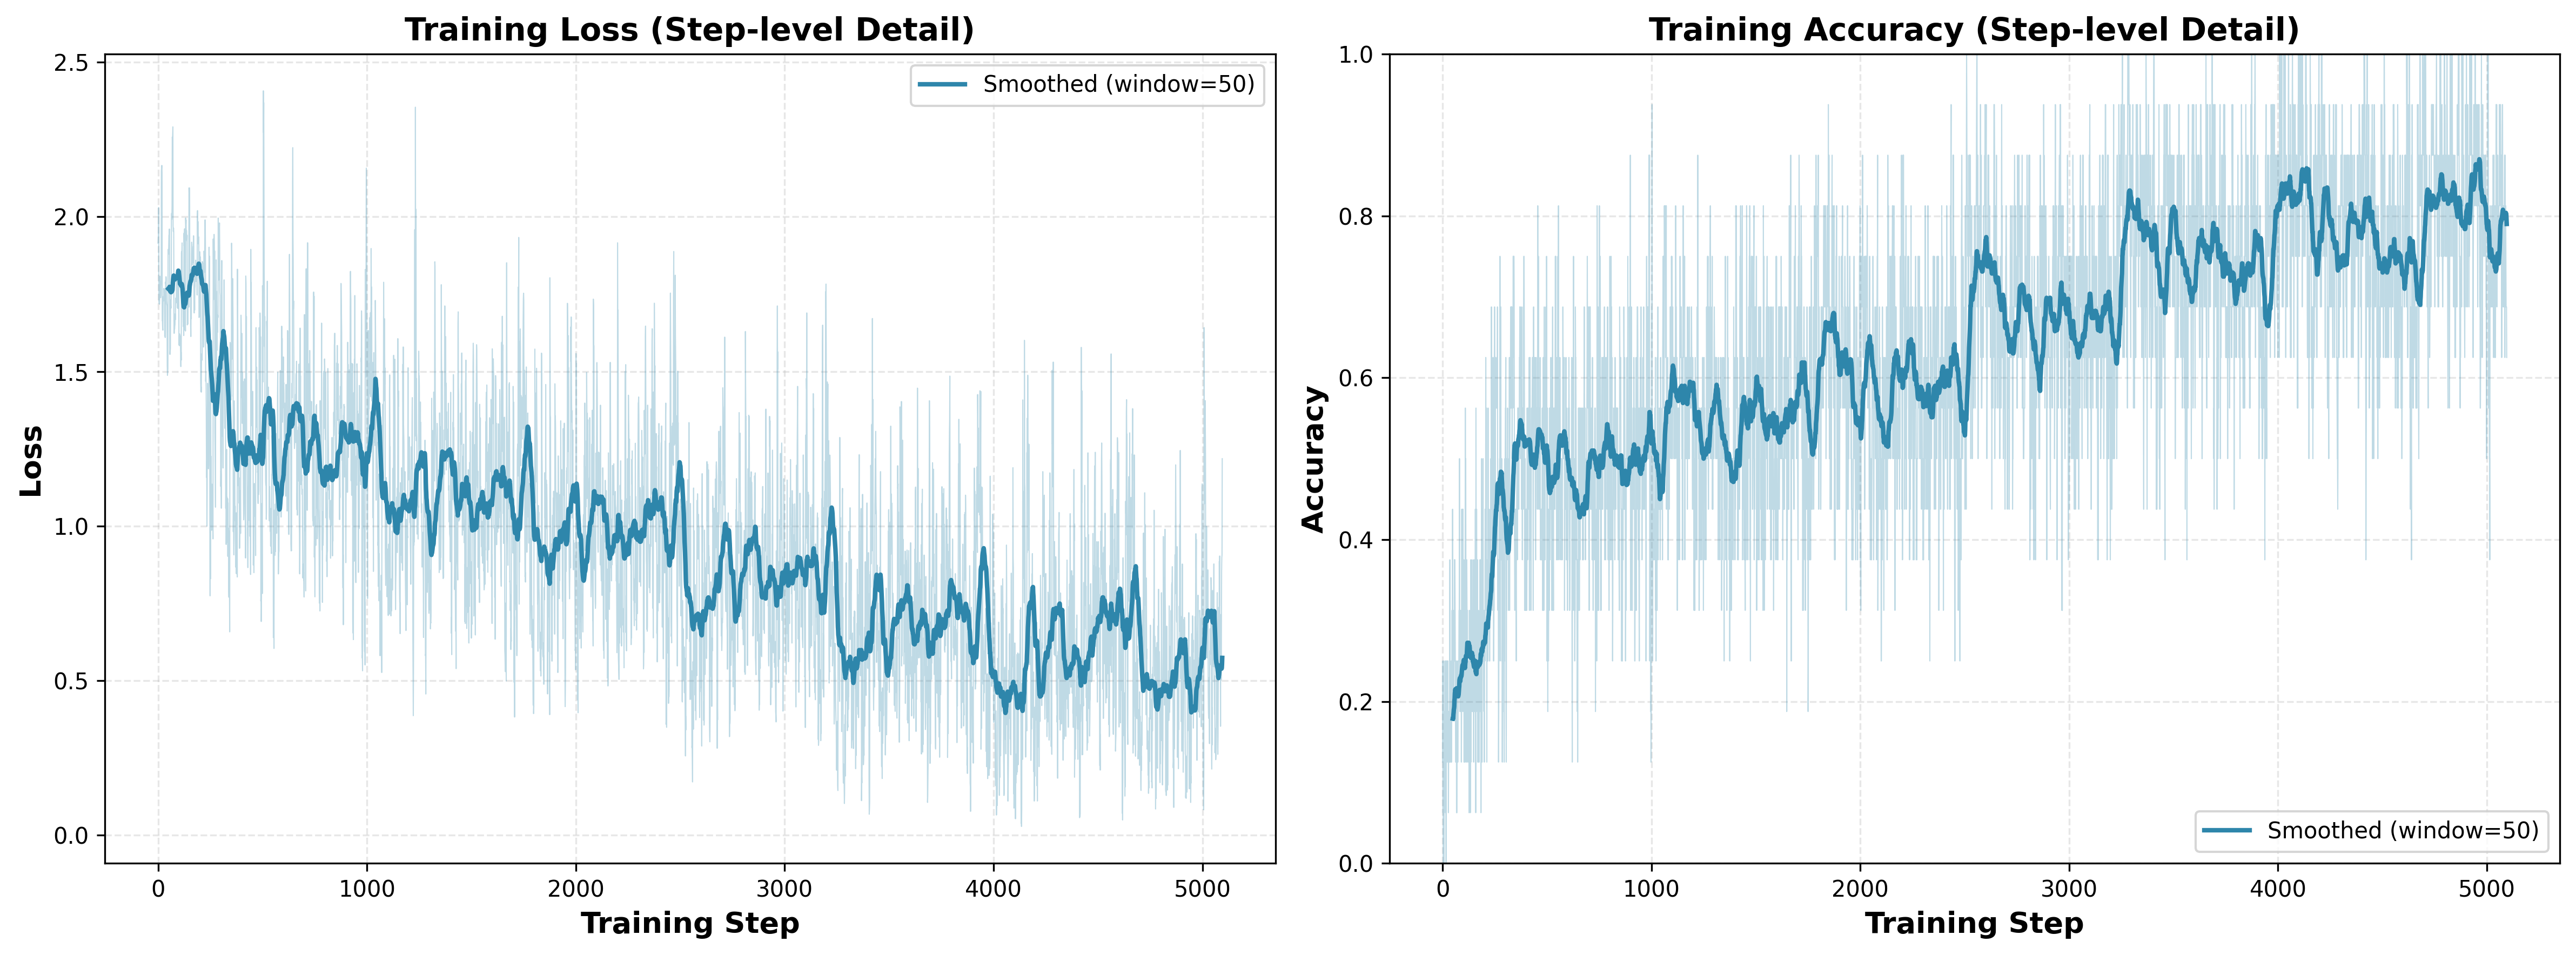
\includegraphics[width=0.85\textwidth]{step_level_plot_cls.png}
\caption{Step-level training dynamics for Cross-Encoder with CLS Pooling.}
\label{fig:step_cls}
\end{figure}

\subsection*{Cross-Encoder with Mean Pooling}
Figure \ref{fig:combined_mp} shows the training and validation performance over epochs for the Mean Pooling model, while Figure \ref{fig:step_mp} presents the step-level training dynamics.

\begin{figure}[H]
\centering
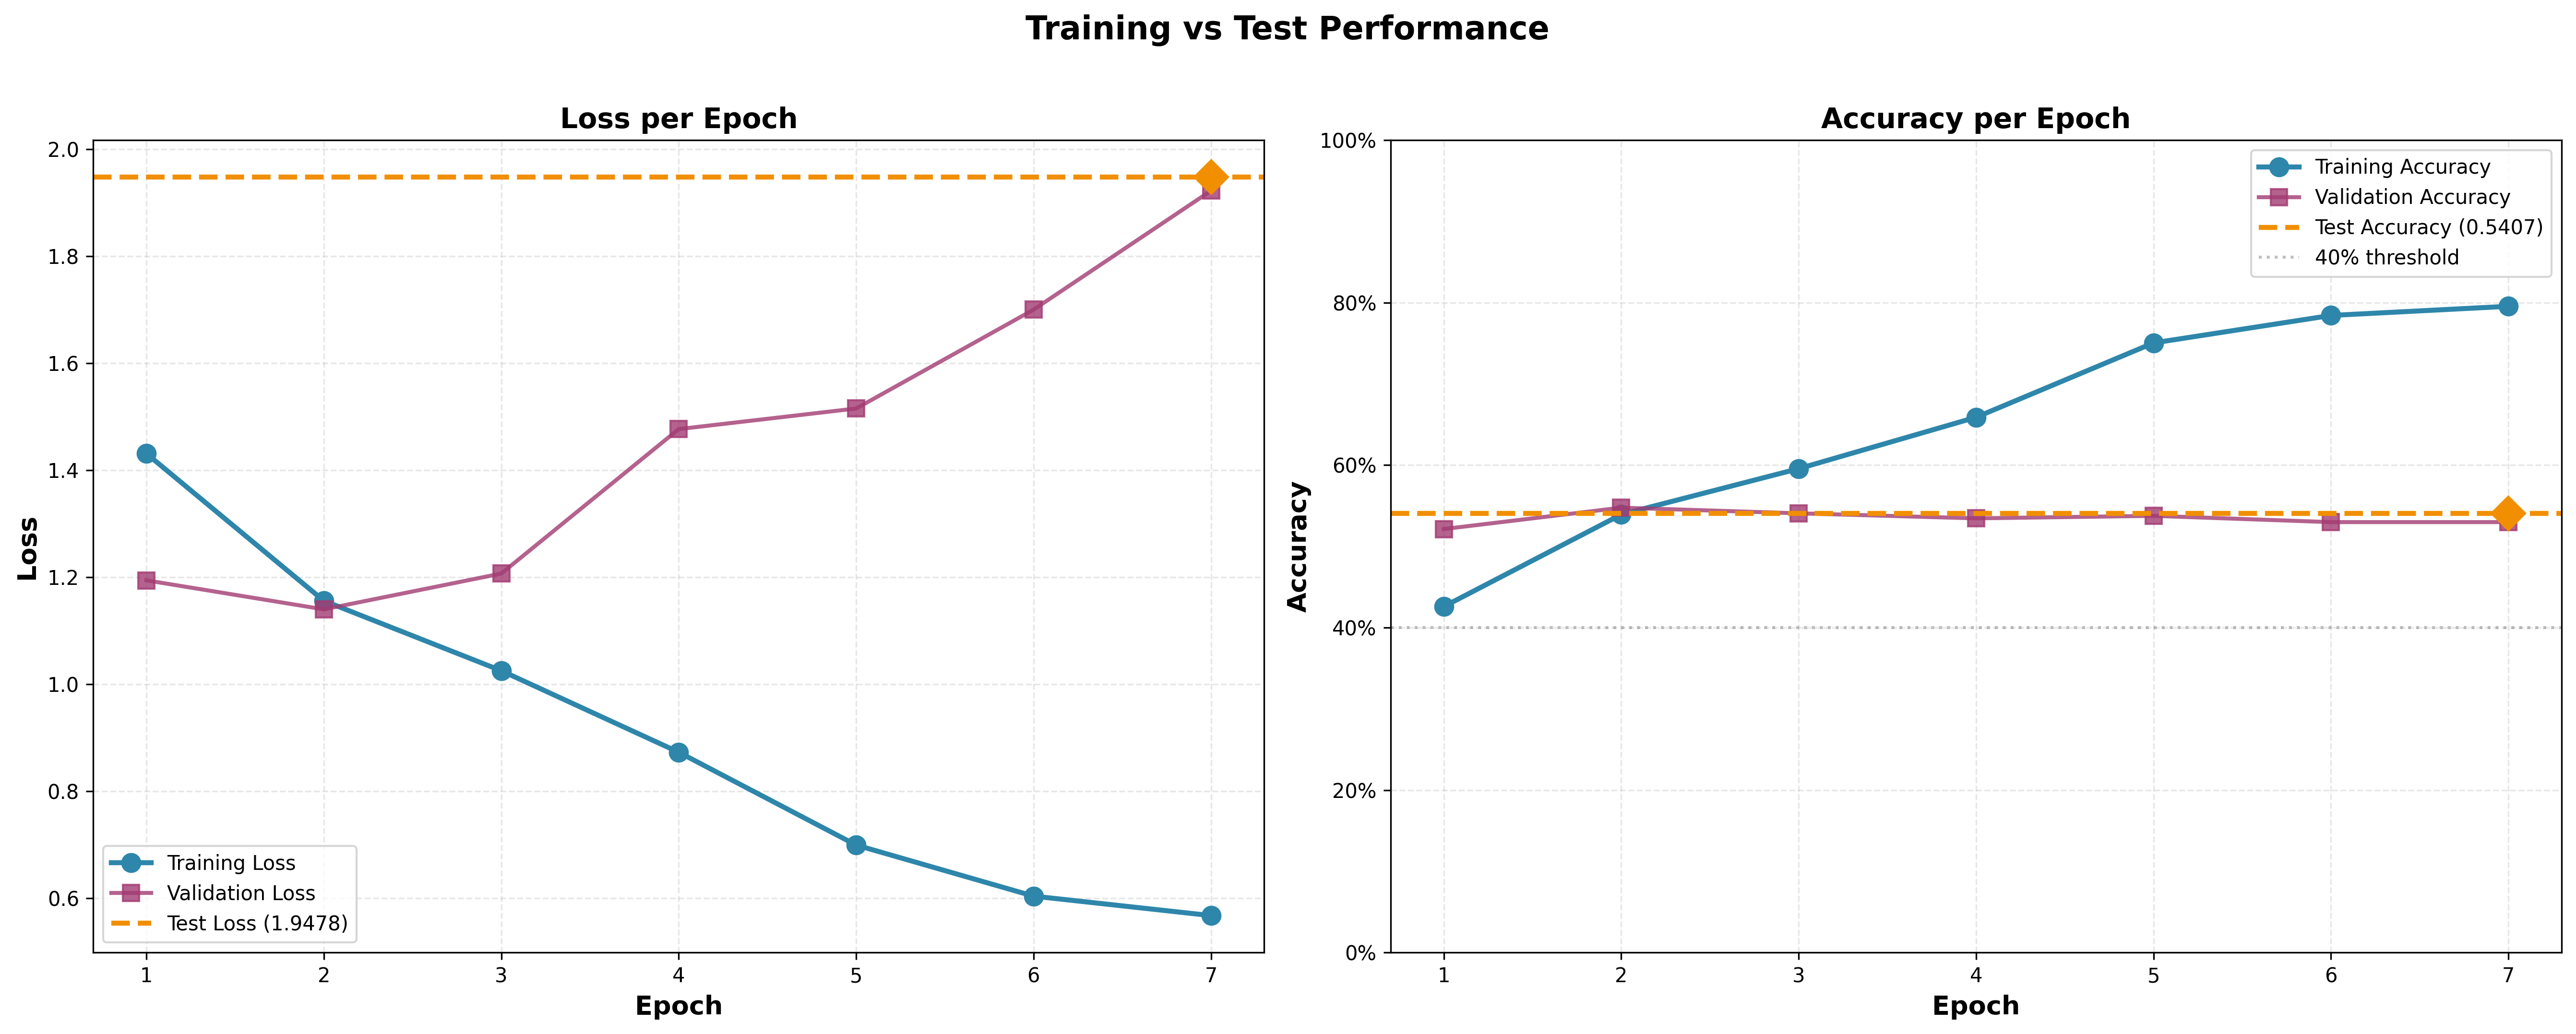
\includegraphics[width=0.85\textwidth]{combined_plot_mp.png}
\caption{Training and validation metrics across epochs for Cross-Encoder with Mean Pooling.}
\label{fig:combined_mp}
\end{figure}

\begin{figure}[H]
\centering
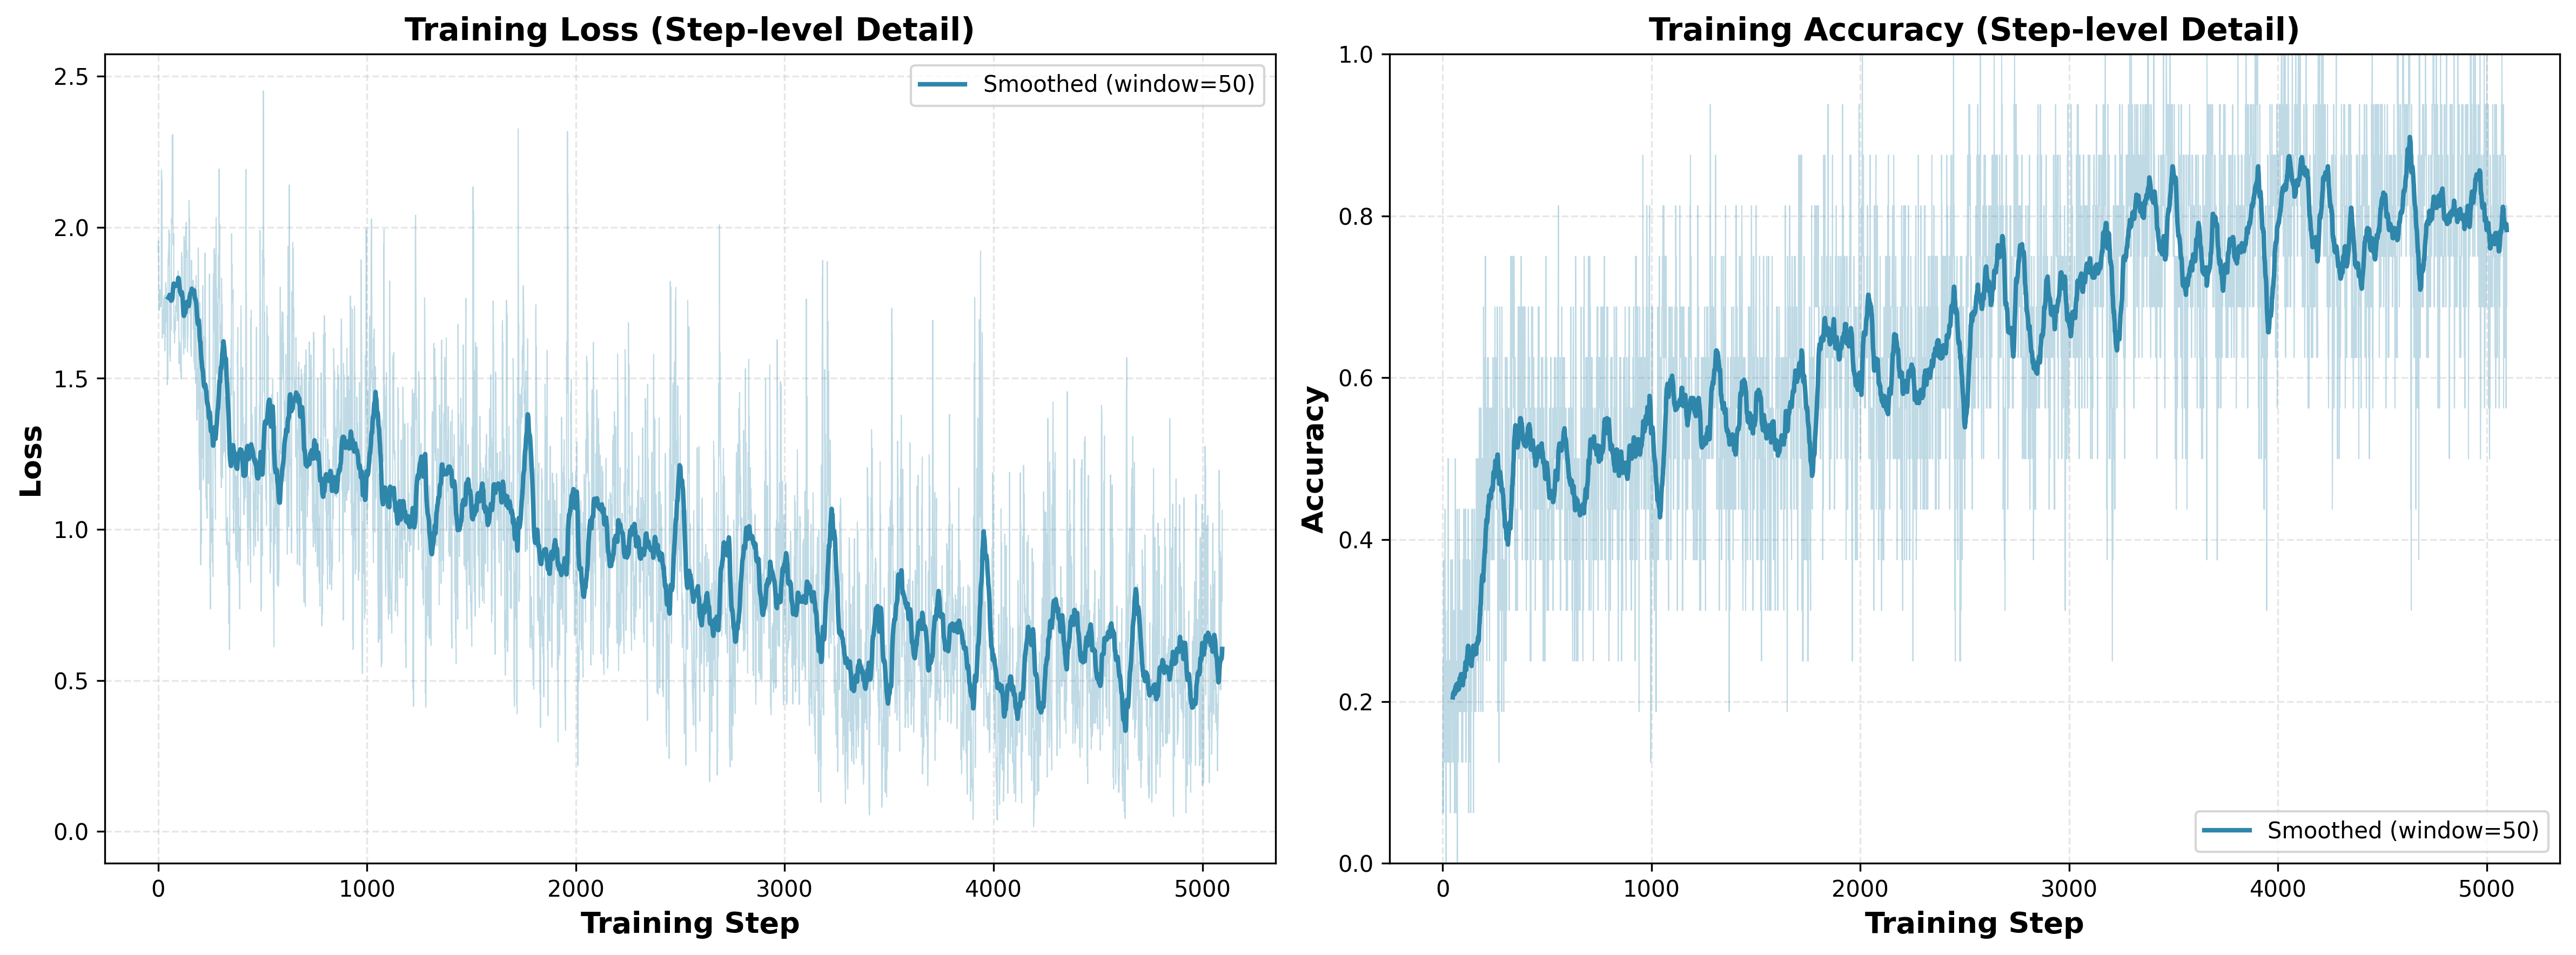
\includegraphics[width=0.85\textwidth]{step_level_plot_mp.png}
\caption{Step-level training dynamics for Cross-Encoder with Mean Pooling.}
\label{fig:step_mp}
\end{figure}

\subsection*{Cross-Encoder with Attention Pooling}
Figure \ref{fig:combined_attn} shows the training and validation performance over epochs for the Attention Pooling model, while Figure \ref{fig:step_attn} presents the step-level training dynamics.

\begin{figure}[H]
\centering
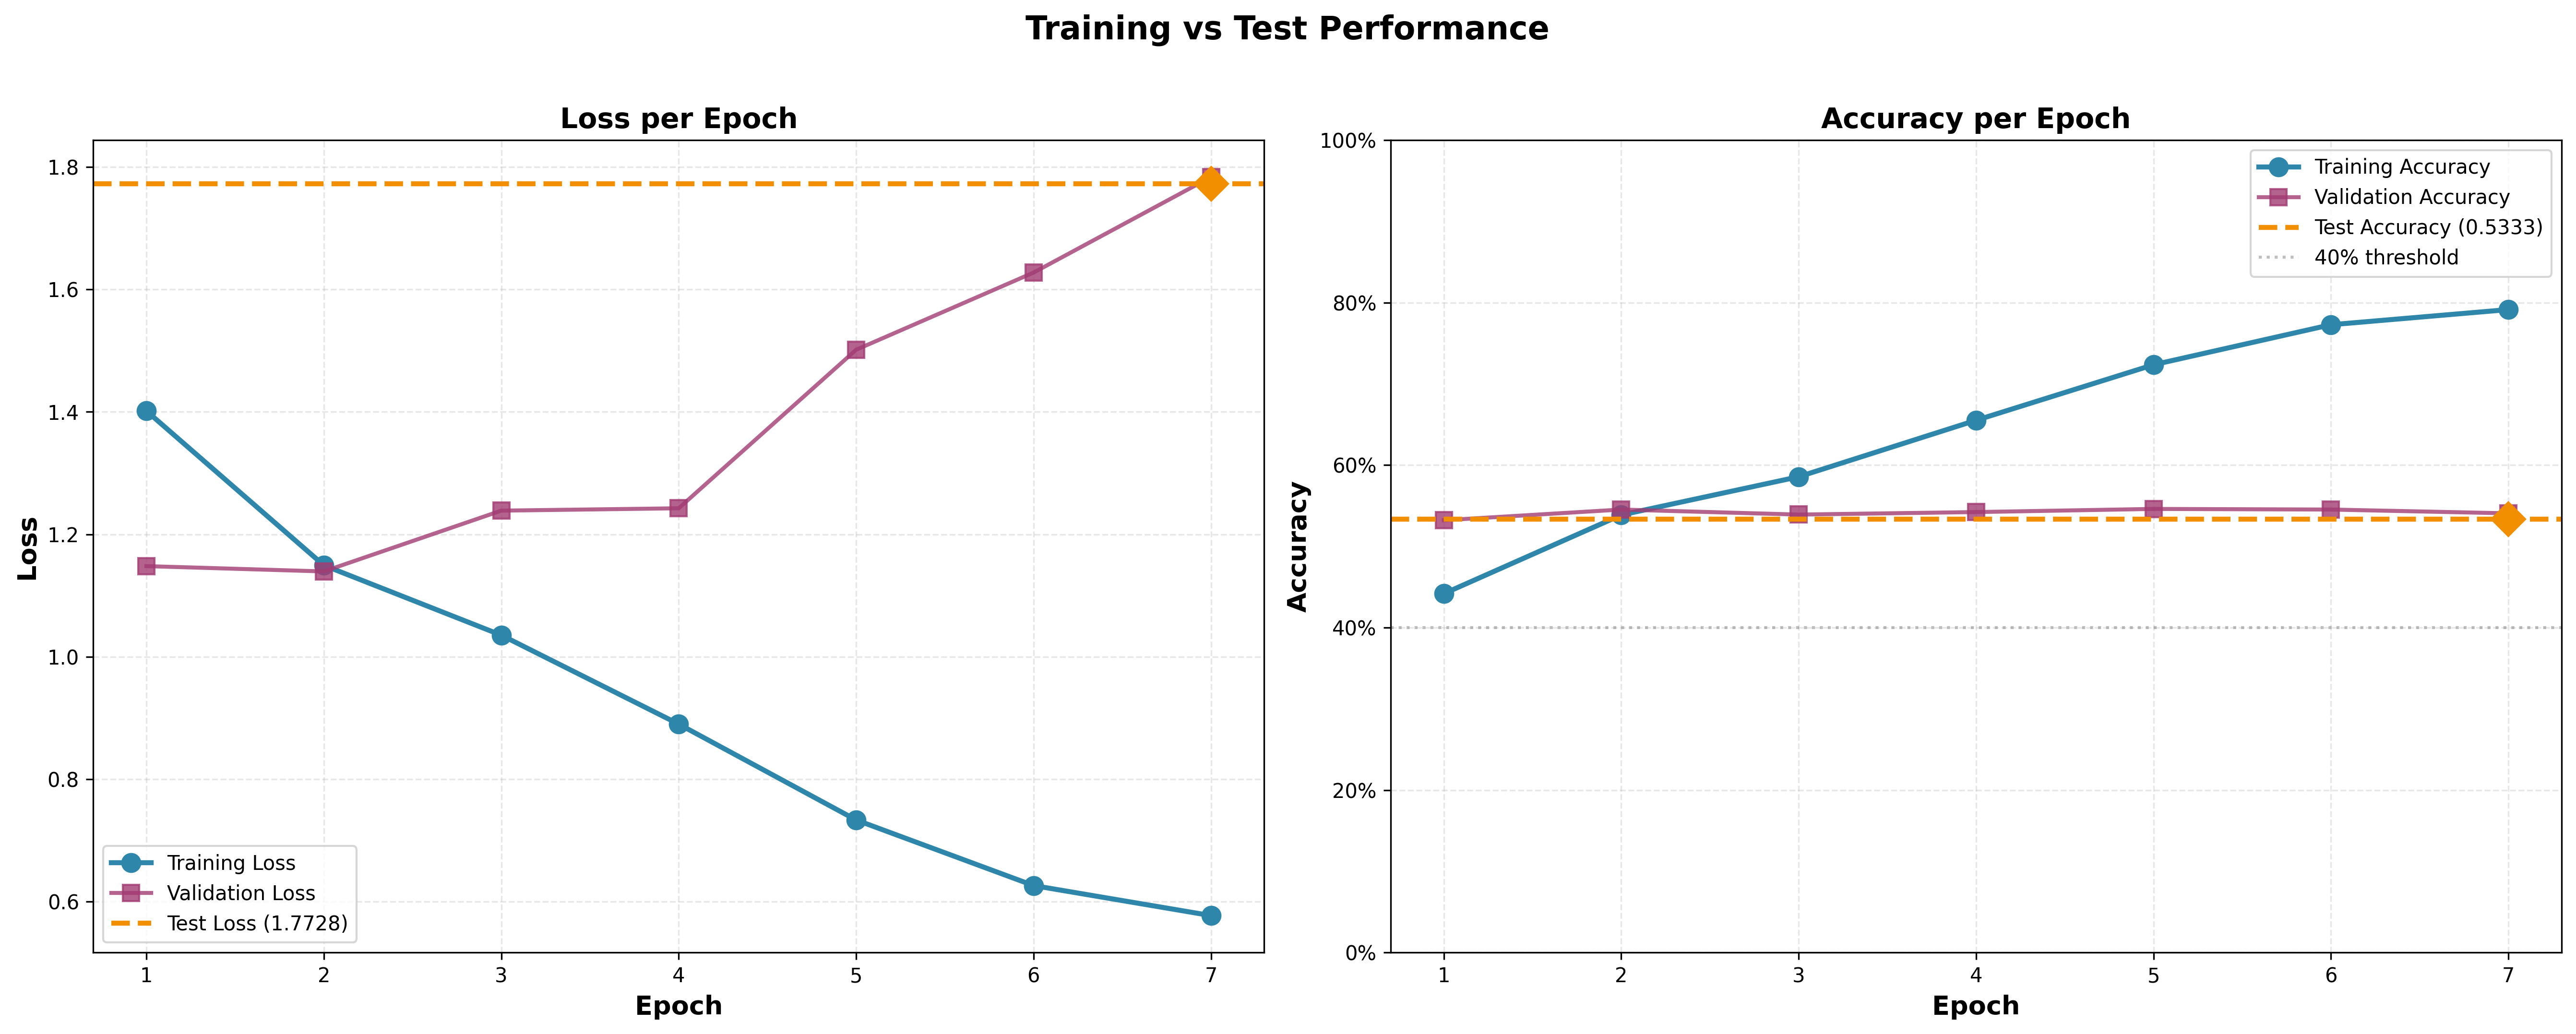
\includegraphics[width=0.85\textwidth]{combined_plot_attn.png}
\caption{Training and validation metrics across epochs for Cross-Encoder with Attention Pooling.}
\label{fig:combined_attn}
\end{figure}

\begin{figure}[H]
\centering
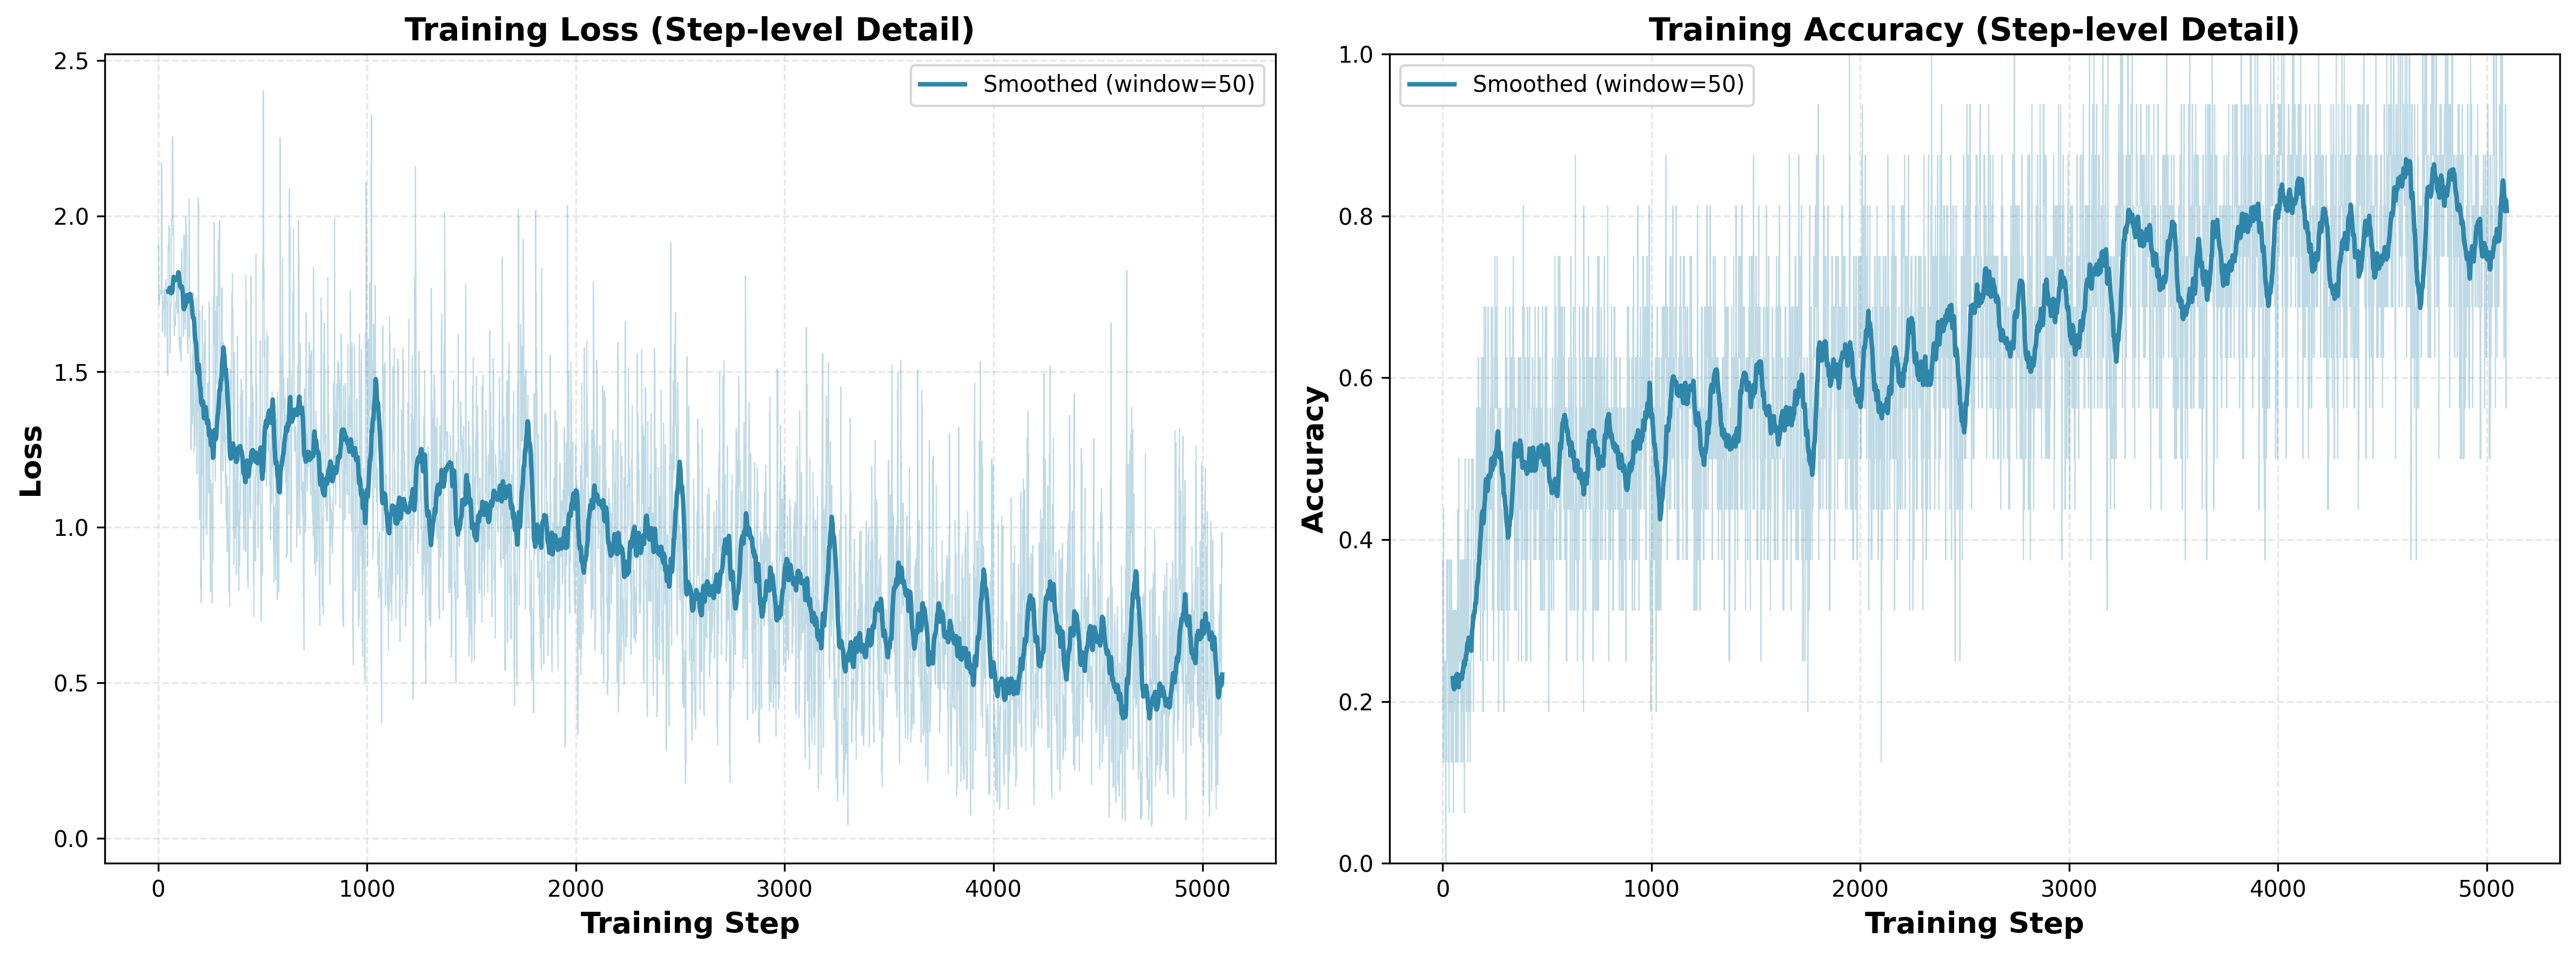
\includegraphics[width=0.85\textwidth]{step_level_plot_attn.png}
\caption{Step-level training dynamics for Cross-Encoder with Attention Pooling.}
\label{fig:step_attn}
\end{figure}

\subsubsection*{Overall Analysis}
Across all three architectures, we observe remarkably similar performance with limited gains from different pooling mechanisms. The test accuracies range narrowly from 0.533 to 0.541, suggesting that the choice of pooling strategy has minimal impact on final ranking quality for this dataset. However, a consistent pattern of overfitting emerges across all models, as evidenced by the substantial discrepancy between training and test losses. While training loss continues to decrease throughout the 7 epochs, the test loss remains significantly higher, indicating that the models are memorizing training-specific patterns rather than learning generalizable representations of query-product relevance. This overfitting behavior could suggest that the current dataset may lack sufficient diversity in query-result pairs to support robust generalization. 

\section*{Conclusion and Future Work}

In this project, we explored various RoBERTa-based cross-encoder architectures for click prediction with assortment in the context of online wine purchasing. Despite experimenting with different pooling strategies, all models achieved similar performance, with test accuracies hovering around 54\%. A notable limitation observed was the pronounced overfitting across all architectures, indicating that the models struggled to generalize beyond the training data.

An important follow-up direction would be to investigate regularization techniques to mitigate overfitting. Similarly, expanding the queries dataset by using LLM to generate synthetic queries through paraphrase augmentation could enhance diversity and improve generalization as demonstrated in \cite{Abaskohi_2023}. Additionally, exploring alternative architectures such as bi-encoders, hybrid models, or ensemble methods that combine cross-encoder and bi-encoder approaches may yield further performance gains. Finally, incorporating additional contextual features, such as user demographics or temporal patterns, could provide richer signals for click prediction.

\bibliographystyle{plainnat}
\bibliography{references}  

\end{document}